\documentclass[17pt]{extarticle}
\usepackage{tikz}

%\newcommand{\dt}[1]{\draw (#1) circle(0.08);}
%For example,  \dt {0,0}

\begin{document}
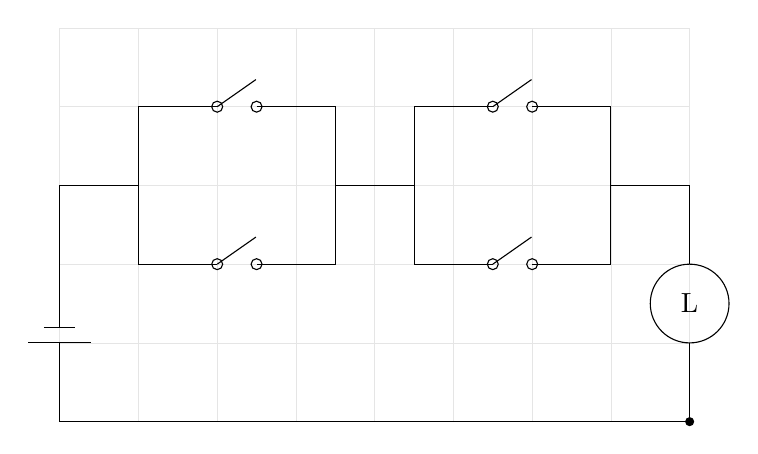
\begin{tikzpicture}[dot/.style={circle,inner sep=1.4pt,draw}]
\draw[very thin, gray!20, step=1 cm](0,0) grid (8,5);
\newcommand{\dt}[1]{\draw (#1) circle(0.07);}
% ------
\draw (0,3) -- (1,3) -- (1,4) --(2,4);

\dt{2,4}
\node [dot] at (2.5,4) {};
\draw (2,4) -- +(35:0.60);

\draw (2.5,4)--(3.5,4) -- (3.5,2)--(2.5,2);
\node [dot] at (2.5,2) {};
\node [dot] at (2,2) {};
\draw (2,2) -- +(35:0.60);

\draw (2,2) -- (1,2) -- (1,3);
%----

\draw (3.5,3) -- (4.5,3) -- (4.5,4) --(5.5,4);

\node [dot] at (5.5,4) {};
\draw (5.5,4) -- +(35:0.60);
\node [dot] at (6,4) {};

\draw (6,4)--(7,4) -- (7,2)--(6,2);
\node [dot] at (6,2) {};
\node [dot] at (5.5,2) {};
\draw (5.5,2) -- +(35:0.60);

\draw (5.5,2) -- (4.5,2) -- (4.5,3);
%----
\draw (7,3) -- (8,3)--(8,2);
\draw (8,1.5) circle(0.5);
\filldraw (8,0) circle(0.05);
\draw (8,1.5)node {L};
\draw (8,1)--(8,0)--(0,0)--(0,1);
\draw (-0.4,1)--(0.4,1);
\draw (-0.2,1.2)--(0.2,1.2);
\draw (0,1.2)--(0,3);

\end{tikzpicture}

\end{document}